%#BIBTEX pbibtex document
% shell_escape_commands = \
% bibtex,bibtex8,\
% kpsewhich,\
% makeindex,\
% mpost,\
% repstopdf,\
% extractbb,\

\documentclass[submit]{ipsj}
%\documentclass[submit,draft]{ipsj}

\usepackage[dvipdfmx]{graphicx}
\usepackage{latexsym}

\usepackage{ctable} % yc
\usepackage{dcolumn} % yc
% \DeclareRelationFont{JY1}{mc}{it}{}{OT1}{cmr}{it}{}
\DeclareRelationFont{JT1}{mc}{it}{}{OT1}{cmr}{it}{}
\DeclareFontShape{JY1}{mc}{m}{it}{<5> <6> <7> <8> <9> <10> sgen*min
    <10.95><12><14.4><17.28><20.74><24.88> min10
    <-> min10}{}
\DeclareFontShape{JT1}{mc}{m}{it}{<5> <6> <7> <8> <9> <10> sgen*tmin
    <10.95><12><14.4><17.28><20.74><24.88> tmin10
    <-> tmin10}{}
\DeclareRelationFont{JY1}{mc}{sl}{}{OT1}{cmr}{sl}{}
\DeclareRelationFont{JT1}{mc}{sl}{}{OT1}{cmr}{sl}{}
\DeclareFontShape{JY1}{mc}{m}{sl}{<5> <6> <7> <8> <9> <10> sgen*min
    <10.95><12><14.4><17.28><20.74><24.88> min10
    <-> min10}{}
\DeclareFontShape{JT1}{mc}{m}{sl}{<5> <6> <7> <8> <9> <10> sgen*tmin
    <10.95><12><14.4><17.28><20.74><24.88> tmin10
    <-> tmin10}{}
\DeclareRelationFont{JY1}{mc}{sc}{}{OT1}{cmr}{sc}{}
\DeclareRelationFont{JT1}{mc}{sc}{}{OT1}{cmr}{sc}{}
\DeclareFontShape{JY1}{mc}{m}{sc}{<5> <6> <7> <8> <9> <10> sgen*min
    <10.95><12><14.4><17.28><20.74><24.88> min10
    <-> min10}{}
\DeclareFontShape{JT1}{mc}{m}{sc}{<5> <6> <7> <8> <9> <10> sgen*tmin
    <10.95><12><14.4><17.28><20.74><24.88> tmin10
    <-> tmin10}{}
\DeclareRelationFont{JY1}{gt}{it}{}{OT1}{cmbx}{it}{}
\DeclareRelationFont{JT1}{gt}{it}{}{OT1}{cmbx}{it}{}
\DeclareFontShape{JY1}{mc}{bx}{it}{<5> <6> <7> <8> <9> <10> sgen*goth
    <10.95><12><14.4><17.28><20.74><24.88> goth10
    <-> goth10}{}
\DeclareFontShape{JT1}{mc}{bx}{it}{<5> <6> <7> <8> <9> <10> sgen*tgoth
    <10.95><12><14.4><17.28><20.74><24.88> tgoth10
    <-> tgoth10}{}
\DeclareRelationFont{JY1}{gt}{sl}{}{OT1}{cmbx}{sl}{}
\DeclareRelationFont{JT1}{gt}{sl}{}{OT1}{cmbx}{sl}{}
\DeclareFontShape{JY1}{mc}{bx}{sl}{<5> <6> <7> <8> <9> <10> sgen*goth
    <10.95><12><14.4><17.28><20.74><24.88> goth10
    <-> goth10}{}
\DeclareFontShape{JT1}{mc}{bx}{sl}{<5> <6> <7> <8> <9> <10> sgen*tgoth
    <10.95><12><14.4><17.28><20.74><24.88> tgoth10
    <-> tgoth10}{}
\DeclareRelationFont{JY1}{gt}{sc}{}{OT1}{cmbx}{sc}{}
\DeclareRelationFont{JT1}{gt}{sc}{}{OT1}{cmbx}{sc}{}
\DeclareFontShape{JY1}{mc}{bx}{sc}{<5> <6> <7> <8> <9> <10> sgen*goth
    <10.95><12><14.4><17.28><20.74><24.88> goth10
    <-> goth10}{}
\DeclareFontShape{JT1}{mc}{bx}{sc}{<5> <6> <7> <8> <9> <10> sgen*tgoth
    <10.95><12><14.4><17.28><20.74><24.88> tgoth10
    <-> tgoth10}{}
\DeclareRelationFont{JY1}{gt}{it}{}{OT1}{cmr}{it}{}
\DeclareRelationFont{JT1}{gt}{it}{}{OT1}{cmr}{it}{}
\DeclareFontShape{JY1}{gt}{m}{it}{<5> <6> <7> <8> <9> <10> sgen*goth
    <10.95><12><14.4><17.28><20.74><24.88> goth10
    <-> goth10}{}
\DeclareFontShape{JT1}{gt}{m}{it}{<5> <6> <7> <8> <9> <10> sgen*tgoth
    <10.95><12><14.4><17.28><20.74><24.88> tgoth10
    <-> tgoth10}{}
\endinput
%%%% end of jdummy.def % フォントに関するWarningを抑制します

\setcounter{巻数}{53}
\setcounter{号数}{10}
\setcounter{page}{1}

\受付{2011}{11}{4}
%\再受付{2011}{7}{16}   %省略可能
%\再再受付{2011}{7}{20} %省略可能
\採録{2011}{12}{1}

\begin{document}
\title{社会人学生を対象とした情報系PBLのための\\
評価モデルの提案}
\etitle{Proposing an evaluation model for PBL students\\
having job experience in Information Systems}

\affiliate{AIIT}{産業技術大学院大学\\
Advanced Institute of Industrial Technology, Shinagawa, Tokyo 140--0011, Japan}
\affiliate{青山}{青山学院大学附置情報科学研究センター\\
Aoyama Gakuin Univ., Information Science Research Center}
%助手

\author{中鉢 欣秀}{Yoshihide Chubachi}{AIIT}[yc@aiit.ac.jp]
\author{中鉢 直宏}{Naohiro Chubachi}{青山}[chubachi@irc.aoyama.ac.jp]

\begin{abstract}
 本研究では社会人学生を対象としたPBLの成績評価モデルとしてのルーブリッ
 クを構築することを目指し,成績評価の実データをテキスト・マイニングする
 ことで特徴的な評価項目を抽出する.形態素解析と基礎的な統計処理により
 PBLにおける教員からの評価の視点の全体的な特性を明らかにすることができ
 たので報告する.
\end{abstract}

\begin{jkeyword}
PBL,成績評価,ルーブリック
\end{jkeyword}

\begin{eabstract}
 In order to develop a rubric as an evaluation model for students in
 IT industries, we obtained significant evaluation items by analyzing
 accumulated evaluation results from PBL with a text mining method. A
 morphological analysis and basic statistics figured out general
 evaluation points by professors.
\end{eabstract}

\begin{ekeyword}
PBL, evaluation model, rubric
\end{ekeyword}

\maketitle

%1
\section{はじめに}
産業技術大学院大学(以下,AIIT)では通常の大学院の修士論文に相当する位
置付けでPBL(Project Based Learning)を実施している\cite{戸沢義%
夫:2007-08-23,酒森潔:2012-05}.情報アーキテクチャ専攻では2008年度より
PBL履修者の成績評価をiPBLと名付けたシステムを用い,データとして蓄積して
いる\cite{中鉢欣秀:2009-05} .

本専攻におけるPBLの成績評価は,学生の活動と成果物に対し,それぞれ質的・
量的側面から点数化することを基本的な方針としている\cite{加藤由花:2009}.
加えて,各教員は学生の講評を記入しており,成績判定会議の資料として用い
ている.

本研究では,この教員による講評のテキスト・データを自然言語解析し,AIIT
における学生の専門的能力の評価の特性を調べることにより,PBLにおいて特に
難しいとされる学生の成績評価モデルの定義を目指している.本学の情報アー
キテクチャ専攻の教授・准教授10名は全て社会人経験を有していることから,
その経験を活かした評価方法の特徴
%業務遂行能力(コンピテンシ)の面で特徴的な評価の方法
や,社会人学生に対する評価の視点などを明らかにしたい.最終的には,
% PBLで学修した実践的な業務遂行能力を評価する場合の質的評価尺度として
% 用いることのできる
「学生に対する講評」として評価されている学習行動の特徴を踏まえ,社会人
学生を対象にした情報系のPBL評価を行う際の学習行動基準を作成することで,
ルーブリック(Rubric)を構築することを狙う.

以下,\ref{sec:背景}.で本研究の背景について述べる.\ref{sec:解析手法}.で
は,対象とした成績評価コーパスの属性と解析手法を示す.\ref{sec:解析結%
果}.では,コーパスが含む専門性の高い単語の抽出結果,及び,品詞毎の出現
頻度のデータを示す.\ref{sec:考察}.では,得られた結果についてルーブリッ
ク作成の観点から考察する.最後に,\ref{sec:結語}.で本稿のまとめを行う.

\section{研究の背景}\label{sec:背景}
近年,実践的な能力育成のためにアクション・ラーニングやPBL(Project
Based Learning)などが盛んに行われている\cite{松澤芳昭:2007,松澤芳%
昭:2008}.このような学習においては,成果だけではなく学習のプロセスを評
価することが必要となる.そのために,ルーブリックという評価手法が注目を
浴びている.ルーブリックの導入事例としては永田ら\cite{永田智子:2003}の
調査による米国コロラド大学ボウルダー校における事例などが紹介されている.

学習にルーブリックを導入することの効果について,鈴木\cite{鈴木雅%
之:2011-12-20}は,学習者に対して事前にルーブリックを提示することで,内
発的動機づけが高くなり,理解を指向して授業を受ける傾向になることを指摘
している.

よって,社会人学生を対象にしたPBL活動においても社会人として求められる評
価の尺度をルーブリックとして提示することで,より学習効果を高めることが
期待できる.しかし,鈴木も指摘している通り,ルーブリックを教育の実践の
中で作り出すことは難しい.本研究で実施している,実際の評価データを解析
することによる体系的なアプローチを一般化することができれば,この問題を
解決するための一助になり得る.

また,AIITで現在行われている文章による講評という評価方法については,教
員ごとの評価の視点にばらつきが生じる恐れが懸念点としてあげられる.また,
学生を評価すべきポイントに漏れが発生することもあり得る.加えて,文章に
よる記述は教員にとって手間がかかる評価方法である.

共通の評価軸としてのルーブリックを構築することができれば,教員による評
価のばらつきを抑えることが期待できる.また,より具体的な評価項目を示す
ことにより,評価ポイントに漏れがないことを確認することもできるようにな
る.加えて,評価軸を体系的に整理した評価表を用意すれば,教員の採点に要
する手間を軽減できる可能性もある.更に,学習者の学習履歴特性を明確に記
録できるようにもなり,学生の将来的なキャリア形成のための資料としても利
用できる\cite{Naohiro2006_1,Naohiro2006_2}.

\section{データの解析手法}\label{sec:解析手法}

今回の解析には,AIITにおける2009年度から2011年度までの3年間分の成績評価
表を対象とすることにした.また,教員が作成した成績表には素点と総合点の
2種類があり,それぞれに講評が記載されている.今回は総合点の講評をデータ
として用いることとした.このデータに含まれる属性を\tabref{tab:属性表}に
示す.なお,事前に教員名と学生名をランダムなIDに置換した.

このデータからコーパスを作成するためにオープンソースの形態素解析ツール
である\texttt{MeCab}\cite{工藤:2004}を用いた.統計処理には
\texttt{R}\cite{R:2012}を使用し,\texttt{MeCab}との連携には
\texttt{RMeCab}\cite{石田:2008}を利用した.

% latex.default(属性表, file = "table/attributes.tex", title = "No",      caption = "分析対象の評価表の属性", label = "tab:属性表",      booktabs = T) 
%
\begin{table}[!tbp]
\caption{分析対象の評価表の属性\label{tab:属性表}} 
\begin{center}
\begin{tabular}{llll}
\toprule
\multicolumn{1}{l}{No}&\multicolumn{1}{c}{属性}&\multicolumn{1}{c}{値}&\multicolumn{1}{c}{備考}\tabularnewline
\midrule
1&教員数&10 名&実務家教員\tabularnewline
2&学生数&150 名&約8割が社会人\tabularnewline
3&評価表の数&12 枚&3年×4Q\tabularnewline
4&評価対象数&587 名&評価した学生数\tabularnewline
5&合計文字数&83428 字&総合評価に記述された文字数\tabularnewline
6&平均文字数&142.1 字&合計文字数 $\div$ 評価対象数\tabularnewline
\bottomrule
\end{tabular}
\end{center}
\end{table}

 % 英語キャプション?

\section{解析の結果}\label{sec:解析結果}

\subsection{専門性の高い単語の抽出}\label{sec:未知語}

専門職大学院におけるPBLの評価の特徴を捉えるため,講評の記述から専門性の
高い単語を抽出する.\texttt{MeCab}で用いているIPA辞書には一般性のある単
語が登録されていると仮定できる.よって,IPA辞書に含まれない未定義語を調
べることにより,一般的な辞書にはない,専門性の高い用語が抽出できること
になる.

まず,\texttt{MeCab}の\texttt{--unk-feature}オプションを用いてテキスト
を解析したところ,239語が未知語となった.これらの大半がカタカナ語とアル
ファベットからなる略語であった.同時に,数値や記号,明らかな誤記やカタ
カナ語の表記の揺らぎも含まれていた.

次に,これらをユーザ辞書に登録した.カタカナ語は一般名詞または固有名詞
として追加した.また,アルファベットからなる略語については,すでに同じ
意味の語がIPA辞書にある場合,または,カタカナ語の未知語として出現してい
た場合,カタカナの表記を基本形としてユーザ辞書に登録した(例:DB → デー
タベース)\footnote{略語で複数の単語として解析し得るものについてはその
まま残した(例:``PM''は``プロジェクトマネジャー''とせず,そのままPMと
して登録した).}.誤記についても,正しい表記を登録した(例:グーループ
→ グループ).カタカナ語の揺らぎは,IPA辞書にある表記を優先して辞書に追
加した(例:スタディー → スタディ).

最後に,未知語と判定された語のうち,199語をユーザ辞書に登録したところ,
数字や記号と誤記による誤判定以外の未知語はなくなった.199語の中から,明
らかな誤記である17語を除外し,残りの182語が専門性の高い用語であると仮定
することにし,これらの語について出現頻度を調べた結果は\tabref{tab:未知%
語頻度結果}となった.

これらは大きくカタカナ語と略語に分けられ,カタカナ語についてはスキル,
リーダシップ,アプリ,マネジャー,レビュー,データベース,フレームワー
ク,アーキテクチャ,コンピテンシ,ドキュメンテーション,クライント,ク
ラウドといった単語が並ぶ.

略語については,PBLやPM(プロジェクトマネジャー)が上位に来るのはデータ
の性格上自然であるが,他にWeb, IT, Java, IPhone, iOS, Android, Skypeと
いった技術用語が多く出現していることが特徴的である.これら以外では,プ
ロジェクトのテーマに含まれるPIA(プライバシー影響評価)やAR(拡張現実感)
等の語が含まれる.

% latex.default(未知語頻度結果, file = "table/michigo_frequency.tex",      title = "ID", caption = "未知語として登録した単語の出現頻度(4回以上)",      label = "tab:未知語頻度結果", booktabs = T) 
%
\begin{table}[!tbp]
\caption{未知語として判定された単語の出現頻度(4回以上)\label{tab:未知語頻度結果}} 
\begin{center}
\begin{tabular}{llllr}
\toprule
\multicolumn{1}{l}{ID}&\multicolumn{1}{c}{Term}&\multicolumn{1}{c}{Info1}&\multicolumn{1}{c}{Info2}&\multicolumn{1}{c}{Freq}\tabularnewline
\midrule
1184&PBL&名詞&一般&$142$\tabularnewline
1187&PM&名詞&一般&$138$\tabularnewline
1327&スキル&名詞&一般&$ 61$\tabularnewline
2223&PIA&名詞&固有名詞&$ 30$\tabularnewline
1506&リーダシップ&名詞&一般&$ 19$\tabularnewline
1244&アプリ&名詞&一般&$ 18$\tabularnewline
1194&Web&名詞&一般&$ 17$\tabularnewline
1463&マネジャー&名詞&一般&$ 15$\tabularnewline
701&レビュー&名詞&サ変接続&$ 14$\tabularnewline
1180&IT&名詞&一般&$ 14$\tabularnewline
1374&データベース&名詞&一般&$ 14$\tabularnewline
1401&ビデオ&名詞&一般&$ 14$\tabularnewline
2257&XDF&名詞&固有名詞&$ 14$\tabularnewline
1418&フレームワーク&名詞&一般&$ 12$\tabularnewline
1250&アーキテクチャ&名詞&一般&$ 11$\tabularnewline
1303&コンピテンシ&名詞&一般&$ 11$\tabularnewline
1379&ドキュメンテーション&名詞&一般&$ 11$\tabularnewline
1280&クライアント&名詞&一般&$ 10$\tabularnewline
1281&クラウド&名詞&一般&$ 10$\tabularnewline
2211&Java&名詞&固有名詞&$ 10$\tabularnewline
1483&モチベーション&名詞&一般&$  9$\tabularnewline
2262&iPhone&名詞&固有名詞&$  9$\tabularnewline
2259&iOS&名詞&固有名詞&$  8$\tabularnewline
1290&コアタイム&名詞&一般&$  7$\tabularnewline
1363&テレビ&名詞&一般&$  7$\tabularnewline
1406&ファシリテータ&名詞&一般&$  7$\tabularnewline
2190&Android&名詞&固有名詞&$  7$\tabularnewline
2244&Skype&名詞&固有名詞&$  7$\tabularnewline
1179&GUI&名詞&一般&$  6$\tabularnewline
1256&インタフェース&名詞&一般&$  6$\tabularnewline
1337&ストリーム&名詞&一般&$  6$\tabularnewline
2187&AR&名詞&固有名詞&$  6$\tabularnewline
1405&ファシリテーション&名詞&一般&$  5$\tabularnewline
2199&DoWMS&名詞&固有名詞&$  5$\tabularnewline
1178&DBMS&名詞&一般&$  4$\tabularnewline
1191&R\&D&名詞&一般&$  4$\tabularnewline
1383&ネゴシエーション&名詞&一般&$  4$\tabularnewline
1419&ブラッシュアップ&名詞&一般&$  4$\tabularnewline
1436&プロマネ&名詞&一般&$  4$\tabularnewline
1442&ベースライン&名詞&一般&$  4$\tabularnewline
1511&レビュー&名詞&一般&$  4$\tabularnewline
2205&Google&名詞&固有名詞&$  4$\tabularnewline
2245&Spring&名詞&固有名詞&$  4$\tabularnewline
2249&Twitter&名詞&固有名詞&$  4$\tabularnewline
2275&協働&名詞&固有名詞&$  4$\tabularnewline
\bottomrule
\end{tabular}
\end{center}
\end{table}

 % tab:未知語頻度結果

ここで作成したユーザ辞書とIPA辞書と併用し,講評の記述に対して形態素解析
を行った.合計で2,774個の形態素が得られ,それらの品詞毎の個数は
\figref{fig:品詞の個数}に示す通りであった.品詞の大半は名詞と動詞で占
められている.次いで,副詞,助詞,形容詞が続いている.

\subsection{名詞についての解析}

最も多く出現した「名詞」について,細分類の内訳を調べたところ
\figref{fig:名詞の細分類}が得られた.ここでは,一般名詞が一番多く,サ変
接続名詞,形容動詞語幹がその後に続く.サ変接続名詞が一般名詞のほぼ半分
の割合で出現している.

\begin{figure}
  \begin{center}
   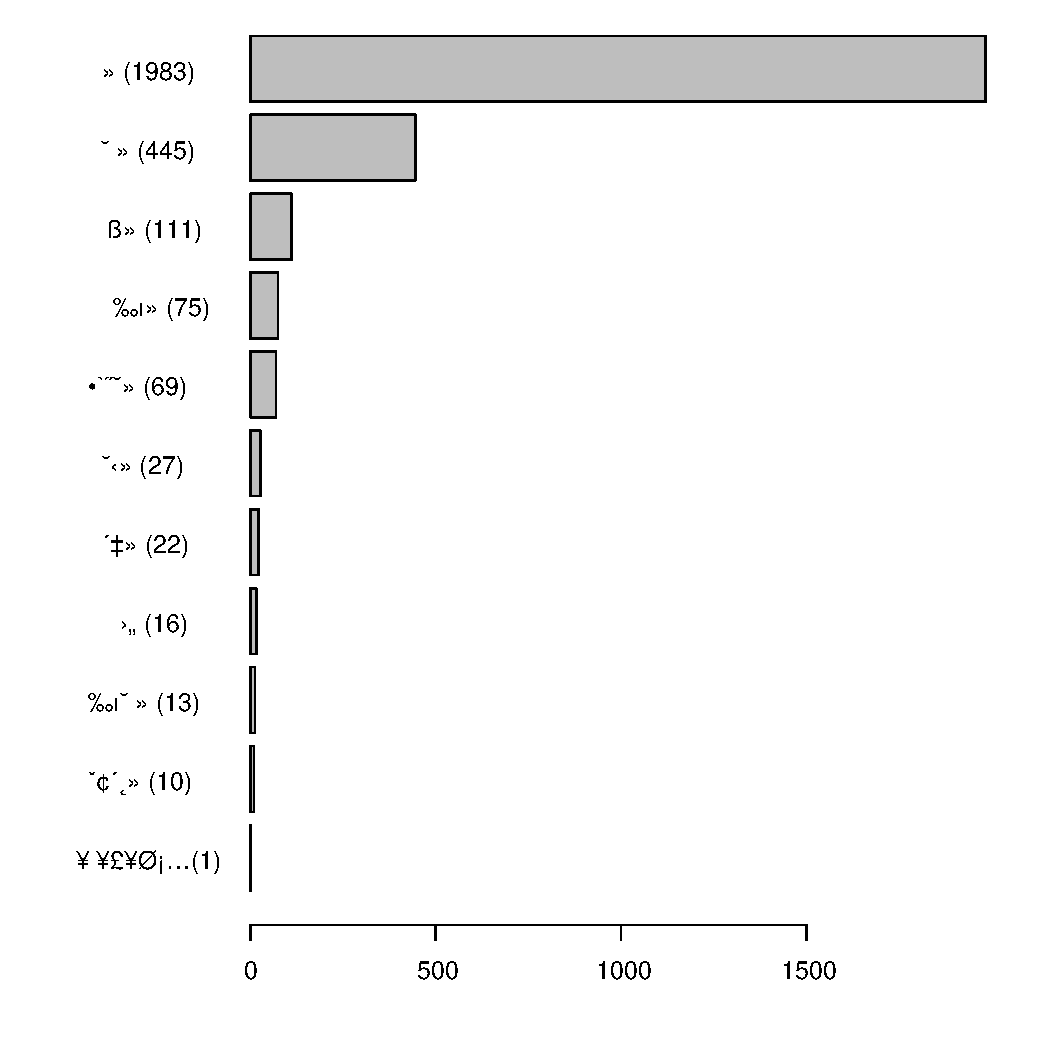
\includegraphics[width=0.8\columnwidth]{R/figure/hinshi.pdf}
  \end{center}
  \caption{講評の形態素解析から得た品詞の個数}
  % \ecaption{!!!Hinshi!!!}
  \label{fig:品詞の個数}
\end{figure}

\begin{figure}
  \begin{center}
   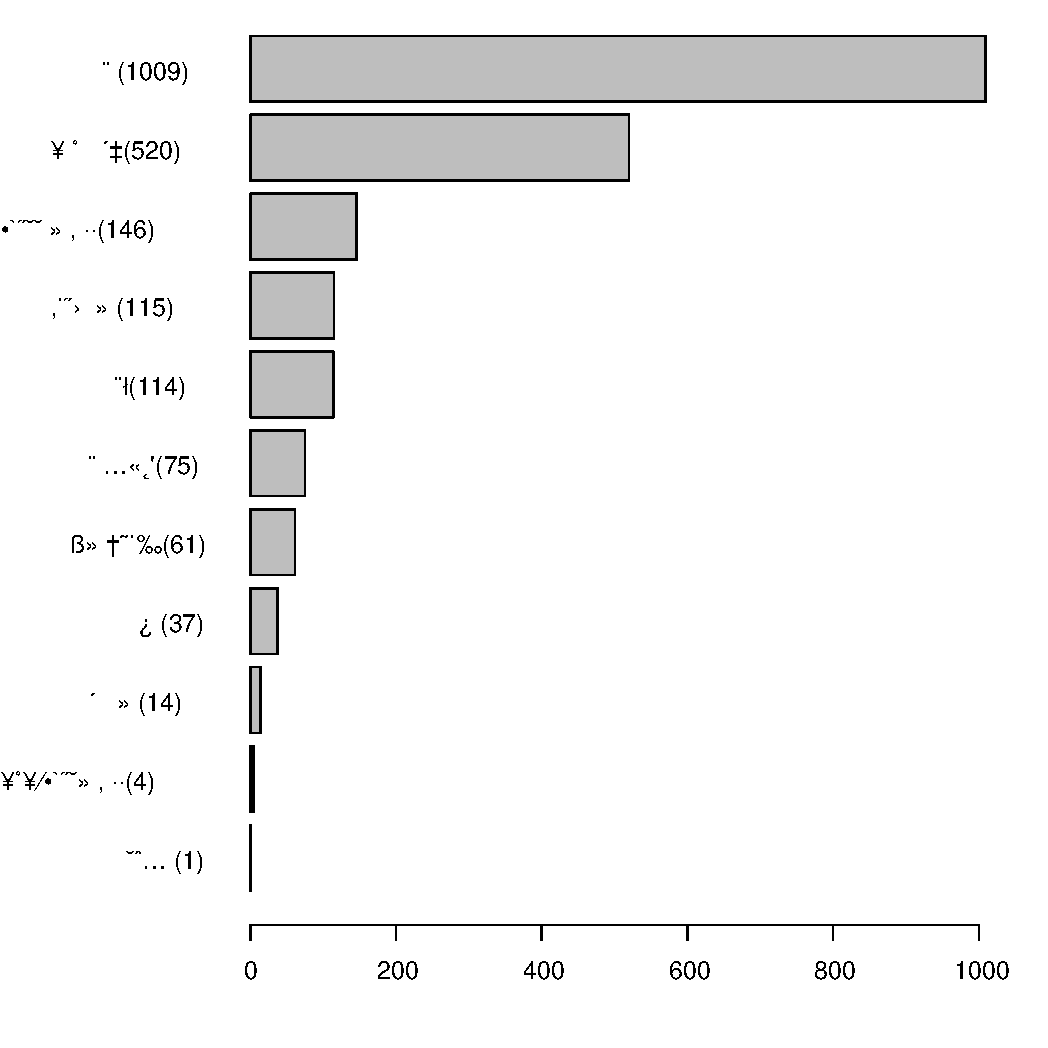
\includegraphics[width=0.8\columnwidth]{R/figure/meishi.pdf}
  \end{center}
  \caption{形態素に出現した名詞の分類}
  % \ecaption{Noun}
  \label{fig:名詞の細分類}
\end{figure}

サ変接続名詞は,「○○する」といった形で動詞的に利用する品詞である.PBLの
評価においては学生または教員などが行った何らかの活動について言及するた
めに用いられている可能性が高い.そこで,このサ変名詞に注目してその詳細
を調べた.

\tabref{tab:サ変接続名詞}に,50回以上の頻度で出現したサ変接続名詞を示し
た.これによると,学生が何らかの活動をしたり,開発をしたり,貢献をした
り,作成をしたりすることについての言及が多くなされていることがわかる.
その一方で,評価する,期待する,といった単語については,主語が教員であ
る可能性がある.よって,これらの単語の使われ方(何を評価するのか,何を
期待するのか)について正確に知るには,共起頻度の解析や係り受けなどを考
慮した解析が必要となる.

% latex.default(頻度表, file = "table/meishi_sahen_50.tex",      title = "ID", caption = "サ変接続名詞の出現頻度(50回以上)",      label = "tab:サ変接続名詞", booktabs = T) 
%
\begin{table}[!tbp]
\caption{サ変接続名詞の出現頻度(50回以上)\label{tab:サ変接続名詞}} 
\begin{center}
\begin{tabular}{llllr}
\toprule
\multicolumn{1}{l}{ID}&\multicolumn{1}{c}{Term}&\multicolumn{1}{c}{Info1}&\multicolumn{1}{c}{Info2}&\multicolumn{1}{c}{Freq}\tabularnewline
\midrule
964&活動&名詞&サ変接続&$356$\tabularnewline
1154&開発&名詞&サ変接続&$281$\tabularnewline
1111&貢献&名詞&サ変接続&$205$\tabularnewline
730&作成&名詞&サ変接続&$203$\tabularnewline
1092&評価&名詞&サ変接続&$198$\tabularnewline
731&作業&名詞&サ変接続&$147$\tabularnewline
898&担当&名詞&サ変接続&$140$\tabularnewline
1039&経験&名詞&サ変接続&$112$\tabularnewline
1104&調査&名詞&サ変接続&$109$\tabularnewline
1004&発表&名詞&サ変接続&$104$\tabularnewline
987&理解&名詞&サ変接続&$103$\tabularnewline
919&提案&名詞&サ変接続&$ 95$\tabularnewline
946&期待&名詞&サ変接続&$ 88$\tabularnewline
804&向上&名詞&サ変接続&$ 87$\tabularnewline
786&参加&名詞&サ変接続&$ 74$\tabularnewline
1108&議論&名詞&サ変接続&$ 71$\tabularnewline
844&対応&名詞&サ変接続&$ 66$\tabularnewline
881&意見&名詞&サ変接続&$ 66$\tabularnewline
949&検討&名詞&サ変接続&$ 63$\tabularnewline
1032&管理&名詞&サ変接続&$ 58$\tabularnewline
955&機能&名詞&サ変接続&$ 57$\tabularnewline
835&実装&名詞&サ変接続&$ 56$\tabularnewline
928&改善&名詞&サ変接続&$ 56$\tabularnewline
1089&設計&名詞&サ変接続&$ 56$\tabularnewline
777&努力&名詞&サ変接続&$ 53$\tabularnewline
953&構築&名詞&サ変接続&$ 50$\tabularnewline
\bottomrule
\end{tabular}
\end{center}
\end{table}

 % tab:サ変接続名詞


\subsection{動詞についての解析}
動詞についても同様に,出現頻度の高いものを調べた.動詞の細分類は
\figref{fig:動詞の細分類}に示した通り,自立語と接尾語と非自立語の3種類
がある.このうち,接尾語と非自立語については単語を見ただけでは性質が分
からないので対象から外し,自立語のみ頻度を調べた.

\begin{figure}[t]
 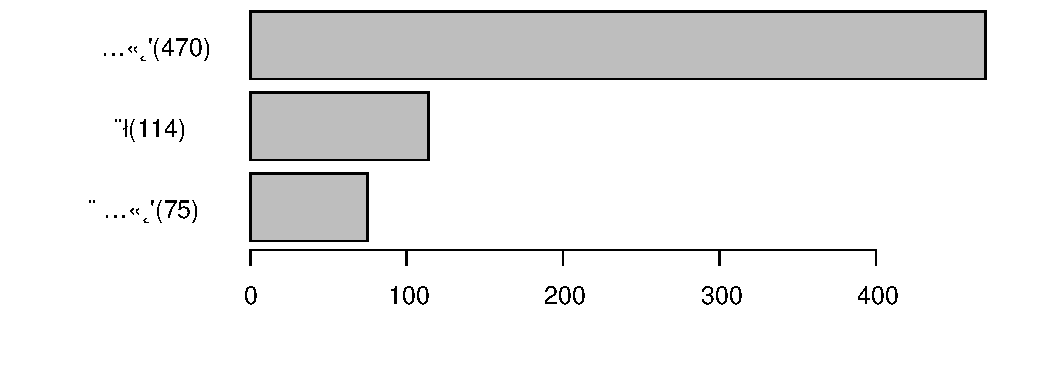
\includegraphics[width=\columnwidth]{R/figure/doushi.pdf}
 \caption{形態素に出現した動詞の分類}
 % \ecaption{Hinshi}
 \label{fig:動詞の細分類}
\end{figure}

講評の文章に15回以上出現した自立動詞を\tabref{tab:自立動詞}に示す.する,
できる,ある,行う等の一般的な動詞以外に着目すると,学生によるPBLでの活
動の状況を記述するために用いられた動詞が含まれていることが分かる.例え
ば,まとめる,取り組む,こなす,すすめる,果たすといった動詞が該当する.

なお,前述のサ変接続名詞に対する解析と同様,それぞれの動詞の主語や目的
語についてはこの結果からだけでは示されない.

% latex.default(頻度表, file = "table/doushi_15.tex", title = "ID",      caption = "自立動詞の出現頻度(15回以上)", label = "tab:自立動詞",      booktabs = T) 
%
\begin{table}[!tbp]
\caption{自立動詞の出現頻度(15回以上)\label{tab:自立動詞}} 
\begin{center}
\begin{tabular}{llllr}
\toprule
\multicolumn{1}{l}{ID}&\multicolumn{1}{c}{Term}&\multicolumn{1}{c}{Info1}&\multicolumn{1}{c}{Info2}&\multicolumn{1}{c}{Freq}\tabularnewline
\midrule
233&する&動詞&自立&$1698$\tabularnewline
248&できる&動詞&自立&$ 337$\tabularnewline
208&ある&動詞&自立&$ 310$\tabularnewline
536&行う&動詞&自立&$ 243$\tabularnewline
258&なる&動詞&自立&$ 175$\tabularnewline
271&まとめる&動詞&自立&$  71$\tabularnewline
353&取り組む&動詞&自立&$  50$\tabularnewline
326&出す&動詞&自立&$  49$\tabularnewline
439&持つ&動詞&自立&$  49$\tabularnewline
229&こなす&動詞&自立&$  44$\tabularnewline
593&進める&動詞&自立&$  40$\tabularnewline
411&得る&動詞&自立&$  38$\tabularnewline
464&果たす&動詞&自立&$  27$\tabularnewline
415&思う&動詞&自立&$  26$\tabularnewline
525&考える&動詞&自立&$  26$\tabularnewline
553&見る&動詞&自立&$  25$\tabularnewline
481&活かす&動詞&自立&$  23$\tabularnewline
500&目立つ&動詞&自立&$  22$\tabularnewline
539&行く&動詞&自立&$  22$\tabularnewline
555&見受ける&動詞&自立&$  19$\tabularnewline
220&かける&動詞&自立&$  18$\tabularnewline
305&伝える&動詞&自立&$  17$\tabularnewline
404&引っ張る&動詞&自立&$  17$\tabularnewline
255&とる&動詞&自立&$  16$\tabularnewline
341&努める&動詞&自立&$  16$\tabularnewline
293&与える&動詞&自立&$  15$\tabularnewline
320&優れる&動詞&自立&$  15$\tabularnewline
387&学ぶ&動詞&自立&$  15$\tabularnewline
497&異なる&動詞&自立&$  15$\tabularnewline
592&進む&動詞&自立&$  15$\tabularnewline
\bottomrule
\end{tabular}
\end{center}
\end{table}

 % tab:自立動詞

\subsection{副詞についての解析}
続いて,副詞についても頻度を解析する.\texttt{MeCab}で作成したコーパス
にある副詞は一般または助詞類接続の2種類に分類されたが,ここでは両者の区
別はしないものとする.

\tabref{tab:副詞}に出現回数が5回以上の副詞をまとめた.全体として,学生
に対して定性的な評価をしている表現が多い.大まかに,肯定的な表現と否定
的な表現に分けるとすると,肯定的な表現としては,よく,きちんと,最も,
極めてなどが該当する.否定的なものとしては,やや,あまり,もう少し,と
いった表現があげられよう.

ただし,副詞は文脈によって指し示す内容が大きく異なるものがある.例えば,
「特に」という語は「特に優れている」と使う場合もあるし,「特に劣ってい
る」という文脈でも使える.従って,これらの副詞による表現の意味を正確に
把握するためには,これらの副詞の前後にくる単語が重要であると考えられる
ので,使用された文脈を踏まえた解析が必要になる.

% latex.default(頻度表, file = "table/fukushi_5.tex", title = "ID",      caption = "副詞の出現頻度(5回以上)", label = "tab:副詞",      booktabs = T) 
%
\begin{table}[!tbp]
\caption{副詞の出現頻度(5回以上)\label{tab:副詞}} 
\begin{center}
\begin{tabular}{llllr}
\toprule
\multicolumn{1}{l}{ID}&\multicolumn{1}{c}{Term}&\multicolumn{1}{c}{Info1}&\multicolumn{1}{c}{Info2}&\multicolumn{1}{c}{Freq}\tabularnewline
\midrule
61&特に&副詞&一般&$42$\tabularnewline
36&よく&副詞&一般&$36$\tabularnewline
35&やや&副詞&一般&$31$\tabularnewline
11&きちんと&副詞&一般&$27$\tabularnewline
37&より&副詞&一般&$27$\tabularnewline
66&あまり&副詞&助詞類接続&$23$\tabularnewline
95&もう少し&副詞&助詞類接続&$22$\tabularnewline
27&ほとんど&副詞&一般&$19$\tabularnewline
91&まだ&副詞&助詞類接続&$17$\tabularnewline
29&もう&副詞&一般&$16$\tabularnewline
53&最も&副詞&一般&$16$\tabularnewline
54&極めて&副詞&一般&$16$\tabularnewline
68&ある程度&副詞&助詞類接続&$16$\tabularnewline
28&ほぼ&副詞&一般&$14$\tabularnewline
9&かなり&副詞&一般&$13$\tabularnewline
72&さらに&副詞&助詞類接続&$13$\tabularnewline
73&しっかり&副詞&助詞類接続&$11$\tabularnewline
102&実際&副詞&助詞類接続&$11$\tabularnewline
96&もともと&副詞&助詞類接続&$ 9$\tabularnewline
32&もっと&副詞&一般&$ 8$\tabularnewline
97&一層&副詞&助詞類接続&$ 8$\tabularnewline
99&全く&副詞&助詞類接続&$ 8$\tabularnewline
101&多少&副詞&助詞類接続&$ 8$\tabularnewline
48&必ずしも&副詞&一般&$ 6$\tabularnewline
98&一応&副詞&助詞類接続&$ 6$\tabularnewline
24&ともに&副詞&一般&$ 5$\tabularnewline
47&徐々に&副詞&一般&$ 5$\tabularnewline
59&比較的&副詞&一般&$ 5$\tabularnewline
70&いろいろ&副詞&助詞類接続&$ 5$\tabularnewline
75&すこし&副詞&助詞類接続&$ 5$\tabularnewline
77&それほど&副詞&助詞類接続&$ 5$\tabularnewline
110&相当&副詞&助詞類接続&$ 5$\tabularnewline
\bottomrule
\end{tabular}
\end{center}
\end{table}

 % tab:副詞

\subsection{形容詞についての解析}

形容詞も自立と非自立に分けることができるが,副詞と同様にこれらの細分類
を区別することなく,頻度を調べた.\tabref{tab:形容詞}に,5回以上出現し
た形容詞を示す.

高い,多いという言葉がよく使われており,学生に対する評価のために頻繁に
用いられていることが分かる.同様に,ない,少ない,という語もよく用いら
れている.これらについても文脈によって内容が変化する(二重否定など)の
で,より詳細な解析が必要であると言えよう.

\section{考察}\label{sec:考察}

今回,解析したデータは専門職大学院の実務家教員によるPBLの成績評価におけ
る実際の資料から得たものである.情報系の専門職大学院であるため,ICT領域
の専門能力に関する評価にやや内容的な偏りがあるものの,PBLという形態の学
習に共通する成績評価軸を定めるための手がかりになる.

% latex.default(頻度表, file = "table/keiyoushi_5.tex", title = "ID",      caption = "形容詞の出現頻度(5回以上)", label = "tab:形容詞",      booktabs = T) 
%
\begin{table}[!tbp]
\caption{形容詞の出現頻度(5回以上)\label{tab:形容詞}} 
\begin{center}
\begin{tabular}{llllr}
\toprule
\multicolumn{1}{l}{ID}&\multicolumn{1}{c}{Term}&\multicolumn{1}{c}{Info1}&\multicolumn{1}{c}{Info2}&\multicolumn{1}{c}{Freq}\tabularnewline
\midrule
2689&高い&形容詞&自立&$145$\tabularnewline
2648&多い&形容詞&自立&$ 78$\tabularnewline
2641&ない&形容詞&自立&$ 77$\tabularnewline
2652&少ない&形容詞&自立&$ 58$\tabularnewline
2649&大きい&形容詞&自立&$ 51$\tabularnewline
2669&無い&形容詞&自立&$ 29$\tabularnewline
2676&良い&形容詞&自立&$ 27$\tabularnewline
2655&弱い&形容詞&自立&$ 22$\tabularnewline
2661&新しい&形容詞&自立&$ 22$\tabularnewline
2697&欲しい&形容詞&非自立&$ 22$\tabularnewline
2694&ほしい&形容詞&非自立&$ 21$\tabularnewline
2642&よい&形容詞&自立&$ 18$\tabularnewline
2633&うまい&形容詞&自立&$ 17$\tabularnewline
2671&粘り強い&形容詞&自立&$ 16$\tabularnewline
2645&低い&形容詞&自立&$ 15$\tabularnewline
2634&おとなしい&形容詞&自立&$ 13$\tabularnewline
2666&深い&形容詞&自立&$ 13$\tabularnewline
2656&強い&形容詞&自立&$ 12$\tabularnewline
2687&難しい&形容詞&自立&$ 10$\tabularnewline
2662&早い&形容詞&自立&$  9$\tabularnewline
2644&乏しい&形容詞&自立&$  8$\tabularnewline
2674&細かい&形容詞&自立&$  8$\tabularnewline
2696&よい&形容詞&非自立&$  8$\tabularnewline
2643&上手い&形容詞&自立&$  7$\tabularnewline
2658&悪い&形容詞&自立&$  6$\tabularnewline
2682&近い&形容詞&自立&$  6$\tabularnewline
2657&忙しい&形容詞&自立&$  5$\tabularnewline
2664&正しい&形容詞&自立&$  5$\tabularnewline
2679&薄い&形容詞&自立&$  5$\tabularnewline
2686&長い&形容詞&自立&$  5$\tabularnewline
2695&やすい&形容詞&非自立&$  5$\tabularnewline
\bottomrule
\end{tabular}
\end{center}
\end{table}

 % tab:形容詞

例えば,\tabref{tab:未知語頻度結果}で示した未知語によるフィルタリングか
ら得た単語のうち,リーダシップや,ドキュメンテーション,モチベーション,
ファシリテーション,ネゴシエーション,レビューといったキーワードは,社
会人の業務遂行能力(コンピテンシ)を評価する観点から,教員が特に意識し
て用いている語である.これらは,PBLの教育効果のメジャメントに一般的に用
いることができうる単語である.

一方で,スキルやコンピテンシといった単語については,これらの語を単独で
見ただけではどのような対象を評価したのかは分からない.しかし,今後,こ
れらのコロケーションを解析することで,これらの単語に共起する語を抽出す
ることができ,具体的にどのようなスキルやコンピテンシが評価されたのかを
調べることができよう.

学生のどのような学習行動が評価の対象となったかということについては,
\tabref{tab:サ変接続名詞}から一定の傾向を見て取ることができる.例として,
「貢献する」という語がサ変接続名詞の出現頻度順位で第3位になっている.こ
れは,学生がチームに対して,何をどのように貢献したかという点が,PBLの評
価において主要な評価の要素になっていることを示す.

加えて,\tabref{tab:自立動詞}で示した自立動詞を見れば,「まとめる」や
「取り組む」といったより具体的な学習行動が記述されていることがわかる.
%これらも,PBL型学習において一般性のある評価項目の候補となり得るだろう.
このような講評が多く見られることは,役割や貢献を評価する社会人のための
PBL評価の特徴である.

\tabref{tab:副詞}と\tabref{tab:形容詞}で示した副詞と形容詞については,
これらの語が用いられた文脈にまで遡らないと評価の項目としては利用しづら
い.しかしながら,将来的には,前後の用語の関係の解析や,これらの単語と
学生の最終的な成績評価の得点との相関関係を調べるなどにより「どのような
評価がされた学生の得点が高くなるのか」といった傾向を分析することができ
る.

\section{おわりに}\label{sec:結語}

本研究では,AIITにおいてPBL型科目を履修した学生の2009年度から3年間分の
成績評価の講評の記述を形態素解析してコーパスを得て,これを元にテキスト・
マイニングを行った.

成績評価コーパスからは,IT系の専門職大学院の社会人学生に対する評価とし
て特徴的な単語を解析できた.これらについて考察したところ,IT系の専門領
域の観点からの評価が多く含まれる一方で,教員が学生の学習行動として期待
し,評価の対象とする内容が抽出できた.学生の実践的な業務遂行能力に関連
するものも多く出現した.

これらの結果から,PBLにおける学生の評価軸として利用できるルーブリックを
構築するための基礎資料として今回の解析結果を用いることができるという感
触を得た.今後,頻出する単語が出現している文脈や,意味内容などについて
より詳細な分析を行い,教員が学生のどんなポイントをどのように評価してい
るのかを明らかにすることを通して,PBL評価のためのルーブリックの構築に反
映させていきたい.

最後に,今回の解析のために用いた成績評価のデータはAIITにおいて実際に行
われた成績評価の実データである.このような実データの解析に基づいての学
生の学習行動の基準化や,それに基づくルーブリックの作成などを行なってい
る事例は少ないと思われるので,この研究の今後の成果についても引き続き公
開していきたい.

\bibliographystyle{ipsjunsrt}
\bibliography{bibliography/chubachi,bibliography/reference}

\end{document}
